\section{Capture and Publication}
\label{sec:capture-publication}

Capture walks the complete private upper tree and converts OverlayFS
representations into typed layer changes.  Regular files become write records
that retain a source path and size so publication can stream their bytes;
symbolic links, directory entries, and empty directories remain typed
entries.  Kernel whiteouts---character devices with device number zero or the
supported whiteout extended attribute---become deletions, while the supported
opaque-directory extended attributes become opaque-directory changes.  An
ordinary name beginning with \texttt{.wh.} is not reinterpreted as a
capture-time marker; it remains a path and is rejected later because that name
space is reserved by the layer format.  Invalid layer paths and unsupported
special files are reported as protected drops rather than silently converted.
Explicit-session publication rejects any such drop.  The lower-level planner
has a narrower exception for an unsupported-special-file drop, so the source snapshot
does not yet justify one uniform protected-drop policy across every
publication entry point.

\begin{figure}[t]
\centering
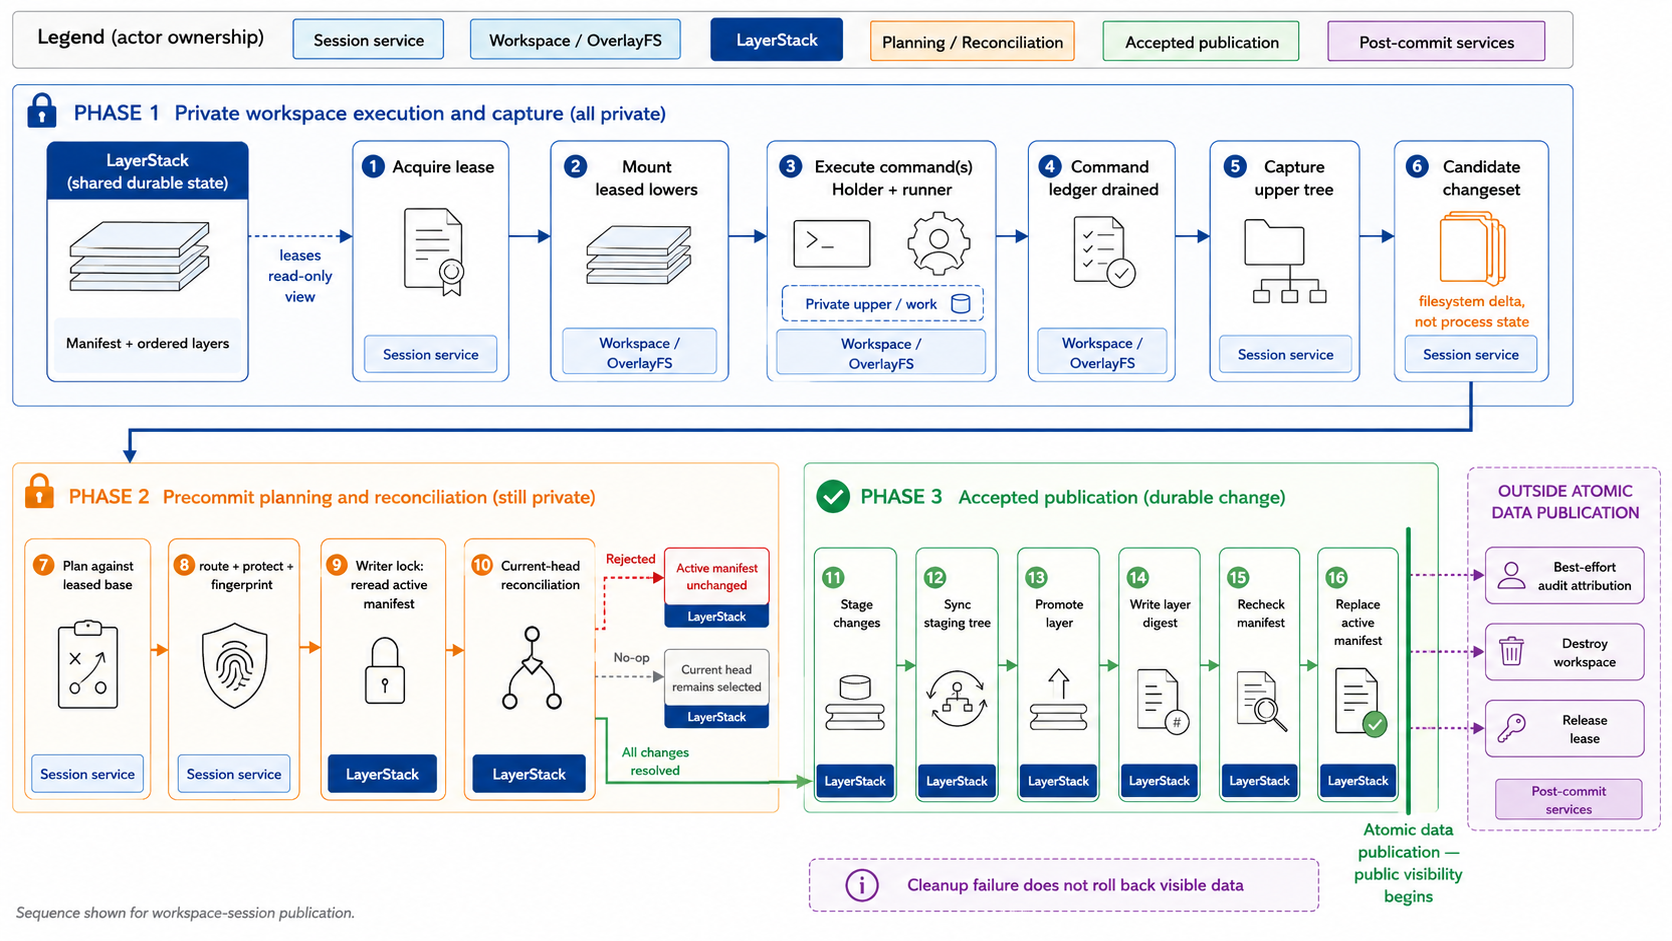
\includegraphics[width=\linewidth]{../figures/concept/fig_publication_sequence.png}
\caption{Workspace-session publication sequence.  Execution, ledger drain,
capture, and current-head reconciliation remain private or precommit.  Public
data visibility begins at active-manifest replacement; best-effort attribution,
workspace destruction, and lease release follow outside the atomic data
publication boundary.  The sequence does not describe sessionless direct file
amendment.}
\label{fig:publication-sequence}
\end{figure}

Planning evaluates the candidate against the leased base before taking the
commit lock.  It verifies that the supplied manifest version, root hash, and
layer count describe the same base manifest.  Each path is then routed as
source or ignored according to the base view's ignore policy, and reserved
runtime paths---including the manifest, layer and staging directories,
\texttt{.layer-metadata}, and \texttt{.wh.*} components---cause rejection.
Source-routed paths receive content fingerprints from the leased base.
Planning an opaque directory additionally enumerates the lower descendants it
would hide: a protected descendant, a mixture of source and ignored routes, or
an expansion beyond the fixed bound rejects the candidate.  These checks turn
a captured delta into an explicit plan; they do not yet make it durable.

The service then acquires the LayerStack writer lock, rereads the active
manifest, and resolves source validations against that current head.  A source
path whose current fingerprint still matches its base fingerprint is accepted
as planned; an idempotent concurrent creation of the same directory is also
compatible.  Changes that replace or obscure a directory trigger descendant
checks so a concurrent change below that path cannot be erased unnoticed.
Other structural differences reject the publication.  Ignored-route changes
are carried as wholesale writes and do not receive the source fingerprint and
merge treatment.  The policy is thus conflict-aware for source state while
making its separate ignored-state route explicit, rather than claiming a
general database isolation level.  Figure~\ref{fig:reconciliation-decision}
expands these route and resolution decisions.

\begin{figure}[t]
\centering
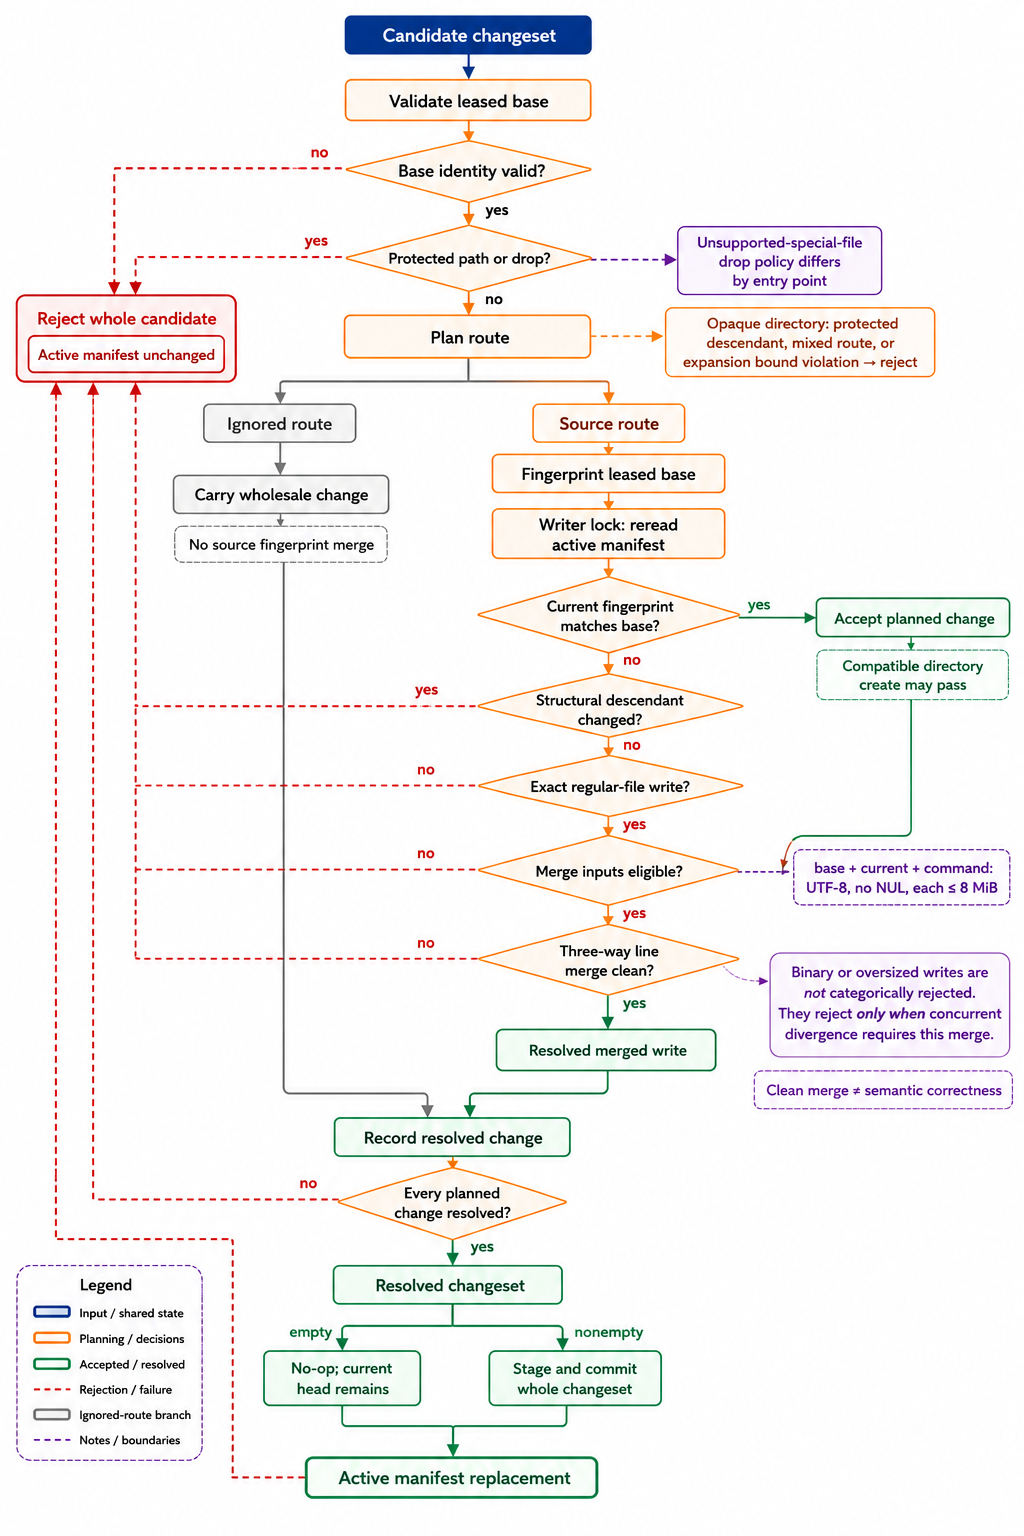
\includegraphics[height=0.82\textheight]{../figures/concept/fig_reconciliation_decision.png}
\caption{Current-head reconciliation decision flow.  Source-routed changes
receive base/current fingerprint and structural checks, and only eligible
exact-file textual divergence reaches three-way line merge.  Every planned
change must resolve before a nonempty changeset is committed; otherwise the
whole candidate is rejected and the active manifest remains unchanged.  A
no-op retains the current head and is not a new data publication.}
\label{fig:reconciliation-decision}
\end{figure}

When a source fingerprint has diverged, the only merge-eligible candidate is a
regular-file write at that exact path.  The resolver reads the leased-base,
current-head, and command versions and applies a three-way line merge only
when each is valid UTF-8 text without NUL bytes and no larger than 8 MiB.
Disjoint edits, or overlapping edits with byte-identical replacement lines,
can yield a clean merged file; differing overlapping edits reject it.  A
non-file transition, binary content, invalid UTF-8, an oversized input, or a
text conflict is ineligible when reconciliation requires this merge and
therefore becomes a source conflict.  By contrast, a binary or oversized
write whose source fingerprint has not diverged can still publish without a
merge.  A clean line merge establishes only structural compatibility: it is
not a semantic-correctness guarantee, and the byte threshold alone is not a
claim that worst-case diff CPU or memory is adequately bounded.

Resolution constructs one final changeset or returns one rejection; no
resolved subset escapes to the layer writer.  Protected paths, invalid base
identity, opaque-directory violations, structural source changes, and
ineligible or conflicting required merges therefore leave the active manifest
unchanged.  An empty resolved changeset is a no-op at the current head.  For an
explicit session, lifecycle handling after a capture or publication failure is
separate from this resolution decision and belongs to
Section~\ref{sec:lifecycle-recovery}.  The data outcomes provide all-or-none
handling without calling the session a full transaction.

For a nonempty resolved changeset, the layer writer first computes its digest
and recognizes an identical current head as a no-op.  Otherwise it writes the
changes beneath a newly allocated staging directory, synchronizes regular
files and the staging tree, renames that tree into the durable layer store, and
synchronizes the layer directory's parent.  It then writes the layer digest,
rereads the active manifest to detect an intervening replacement, and builds a
new manifest whose first entry is the promoted layer.  The manifest writer
creates and synchronizes a temporary file, renames it over the active manifest,
and synchronizes the containing directory.  Only this final replacement makes
the resolved layer part of the active head.  Failures before it can leave
recoverable staging or unreferenced artifacts, but they do not select the new
layer in the active manifest.

The successful manifest replacement is the end of \emph{atomic data
publication}, not the end of the session lifecycle.  After the layer commits,
the operation service maps structural line origins to an owner and appends
per-path audit events.  That attribution is deliberately best effort: an audit
append failure does not fail or roll back the visible data.  The service then
begins the separate workspace-destruction and lease-release phase.  Accounting,
observability events, autosquash notification, session cleanup, and later
garbage collection likewise remain outside the all-or-none data boundary;
Section~\ref{sec:lifecycle-recovery} defines their failure outcomes.

This path explains how one private filesystem delta can become one durable
public head at the audited Linux source snapshot. It does not establish
semantic merge correctness, a cross-platform crash proof, or an unlimited
transaction size. Staging remnants, retained sessions, lease release, cleanup
failure, compaction, and reclamation are lifecycle and recovery concerns,
which Section~\ref{sec:lifecycle-recovery} treats separately.

\clearpage
